
%(BEGIN_QUESTION)
% Copyright 2015, Tony R. Kuphaldt, released under the Creative Commons Attribution License (v 1.0)
% This means you may do almost anything with this work of mine, so long as you give me proper credit

Sketch arrows next to each of the two solenoid valves showing the directions of air flow in the energized (E) and de-energized (D) states, assuming both of the solenoid valves must ``trip'' in order to force the process valve to go to its ``fail'' position (i.e. 2oo2 to trip):

$$\includegraphics[width=15.5cm]{i00982x01.eps}$$

\underbar{file i00982}
%(END_QUESTION)





%(BEGIN_ANSWER)

$$\includegraphics[width=15.5cm]{i00982x02.eps}$$
 
%(END_ANSWER)





%(BEGIN_NOTES)


%INDEX% Final Control Elements, valve: fail-safe solenoids
%INDEX% Process: incinerator (realistic P&ID shown)

%(END_NOTES)


